\section{Discussion}
The results obtained in \Cref{sec:results} are summarized in Table \ref{tab:sim_res_worlds} and Table \ref{tab:sim_res_worlds_active}.
\begin{center}
  \captionof{table}{Simulation results for all environments without active dispersion.\label{tab:sim_res_worlds}}
  \begin{tabular}{c|cc|cc|cc|ccc}
    Environment & 3 agents & & 6 agents & & 15 agents & & 50 agents\\
    \hline
    Coverage & Initial & Final & Initial & Final\ & Initial & Final\ & Initial & Final\\
    \hline
    Tinyworld   & 100\% & 100\% & - & - & - & - & - & - \\
    Tinyworld2  & 65.9\% & 71.8\% & 82.5\% & 98\% & - & - & - & - \\
    Rectworld   & 8\% & 22.1\%& 10\% & 25.5\% & 15\% & 95\% & - & - \\
    Complexworld& - & - & - & - & - & - & 7.5\% & 15.5\% \\
\end{tabular}
\end{center}

\begin{center}
  \captionof{table}{Simulation results for all environments with active dispersion.\label{tab:sim_res_worlds_active}}
  \begin{tabular}{c|cc|cc|cc|ccc}
    Environment & 3 agents & & 6 agents & & 15 agents & & 50 agents\\
    \hline
    Coverage & Initial & Final & Initial & Final\ & Initial & Final\ & Initial & Final\\
    \hline
    Tinyworld   & 100\% & 100\% & - & - & - & - & - & - \\
    Tinyworld2  & 65.9\% & 45.2\% & 82.5\% & 100\% & - & - & - & - \\
    Rectworld   & 8\% & 25\%& 10\% & 46\% & 15\% & 93\% & - & - \\
    Complexworld& - & - & - & - & - & - & 7.5\% & 89\% \\
\end{tabular}
\end{center}
%\subsection{Percentage of coverage}
%As seen in Table \ref{tab:sim_res_worlds} and \ref{tab:sim_res_worlds_active}, there are no consistent results showing 
%wether or not Algorithm \ref{alg:alg1} yields a higher percentage of coverage with or without active dispersion. Not applying active dispersion
%means the local objective for all agents is simply the local probability of coverage. Using active dispersion the local objective
%is a combination of local probability of coverage and dispersion. With this in mind it would make sense if Algorithm \ref{alg:alg1}
%yielded higher percentage of coverage when active dispersion is not applied, as all agents solely focus on maximizing their local probability of coverage.
%The reasons why this is not the case is due to active dispersion forcing agents to explore.
\subsection{Coverage percentage of feasible space}
As the results in Table \ref{tab:sim_res_worlds} show, running Algorithm \ref{alg:alg1} without active dispersion yields configurations where the 
final coverage is always equal to or better than the initial coverage in terms of coverage percentage. The only environment in which the coverage is not approved upon is the Tinyworld environment.
This is due to the Tinyworld environment being constructed so that, in any configuration, 3 or more agents cover the entire feasible space.

When applying active dispersion Algorithm \ref{alg:alg1} returns configurations where the final coverage percentage is higher than the initial coverage percentage in all environments
except for the Tinyworld2 environment. The reason for the diminishing percentage of coverage in the Tinyworld2 environment is discussed in \Cref{secc:improp_weight_disc}.

\subsection{Clustering}
In all simulations, agents tend to gather in groups of three, and cluster as closely together as the constraints \eqref{min_dist_neigh}-\eqref{non_linear_neighb} allow.  
This behavior is especially prevalent when there are not enough agents to cover the entire feasible space, and when active dispersion is not applied. This a consequence 
of the area of the intersection of three circles being largest when the circle centers coincide. Considering the results in \cite{CRB_multilat} such behavior is disadvantageous. The region in which
the accuracy of multilateration (in presence of measurement noise) is the greatest lies in and around the convex hull of the agents. Tight clustering yields a small convex hull, 
meaning the region in which accurate multilateration can be performed is small.


\subsection{Active dispersion as cluster prevention}
In the Tinyworld environment, whose simulation results are shown in \Cref{secc:tinyworld}, the effect of active dispersion is evident (\figref{fig:3_agnt_tw_k_1_0_distr} and \figref{fig:3_agnt_tw_k_1_1_k_2_1_distr}). 
In the case where no active dispersion is used the objective function is constant over the feasible space. Hence the initial configuration is one of 
infinitely many equal valued optima, and Algorithm \ref{alg:alg1} halts after one iteration. In the case where active dispersion is applied the agents spread to the corners of the
feasible space as seen in \figref{fig:3_agnt_tw_k_1_1_k_2_1_distr}. This is due to the fact that the local probability of coverage is constant over the feasible space for all agents, hence the 
local optimization problem \eqref{local_opt_prob} is equivalent to maximizing dispersion between an agent $a$ and its neighbors. 

Simulations performed in the Rectworld environment for 15 agents exhibit some of the same behavior. The final configuration obtained when active dispersion
is applied is shown in \figref{fig:15_agnt_bw_k_1_1_k_2_1_distr}. Comparing this to the configuration obtained in the same environment with the same number of agents (see \figref{fig:15_agnt_bw_k_1_0_k_2_1_distr}), 
it is clear that the agents are more evenly spread out in the mission space when active dispersion is used. In densely populated areas the gradient of the local probability of coverage tends to be small. This is due to the fact that in densely populated areas, 
the majority of the area is covered independently of an agent $a$ covering it or not. Thus any small perturbation of an agent's position does not have a major impact on
the agent's local probability of coverage. As the number of neighbors for an agent in a densely populated area is large, the dispersion term is significantly negative and has a steep gradient.
This combination of movement having a small impact on the local probability of coverage and a large impact on the value of the dispersion term causes agents to move away from densely populated areas, 
preventing clustering. The coverage percentage is however two percent smaller when using active dispersion for a swarm of 15 agents in the Rectworld area than when only optimizing the local probability of coverage.

Active dispersion does however not prevent clustering in sparsely populated areas. This can be seen by the configurations for 3 and 6 agents in the
Rectworld environment (\Cref{fig:3_agnt_bw_k_1_1_k_2_1_distr} and \Cref{fig:6_agnt_bw_k_1_1_k_2_1_distr}). In these configurations, any
movement from the current configuration would cause the local
probability of coverage for the agent that moves to drop significantly. Furthermore, none of the agents have enough neighbors to force them to move despite
the drop in local probability of coverage.

\subsection{Effect of improperly weighted active dispersion}\label{secc:improp_weight_disc}
The simulations performed for a swarm of size 3 in the Tinyworld2 environment display a weakness of active dispersion. Here the swarm covers a significantly smaller percentage of the 
feasible space when applying active dispersion than when not. This is due to the fact that the dispersion term is weighted too heavily. When the local probability of coverage for an agent is small, i.e. $L(\mathbf{X}_{\mathcal{B}_{a}\cup\{a\}})$ is small 
for all possible values of $\mathbf{x}_{a}$, the value of 
the local objective \eqref{totally_objective} is dominated by the dispersion term. This causes a shift in behavior. The focus is on dispersion rather than coverage, and Algorithm \ref{alg:alg1} converges
to a solution that gives a smaller coverage percentage.

For a swarm of 6 agents in the Tinyworld2 environment, the case is quite different. Now active dispersion yields a configuration that gives a larger coverage percentage than when no active
dispersion is applied. This result is although not a consequence of clever objective function formulation. As for three agents, the active dispersion term dominates the coverage term
in \eqref{totally_objective} due to the local probability of coverage being small no matter the value of $\mathbf{x}_{a}$. Hence the agents focus on maximizing dispersion rather than covered area. The 
solution generated by Algorithm \ref{alg:alg1} for 6 agents in the Tinyworld2 environment is identical to the solution generated for 6 agents in the Tinyworld environment when applying active dispersion. 
This makes it obvious that the high percentage of coverage obtained in the Tinyworld2 environment using active dispersion is not caused by the agents meticulously positioning themselves in order to maximize the local
probability of coverage. Instead, they position themselves so that the maximum dispersion is obtained, and the higher percentage of coverage is obtained coincidentally.

\subsection{Active dispersion forcing exploration}
\figref{fig:6_agnt_bw_k_1_0_k_2_1_distr} shows the configuration obtained
by running Algorithm \ref{alg:alg1} for a swarm of size 6 in the Rectworld environment  without active dispersion. The three agents in the bottom-left corner stay
at their initial positions throughout the simulation even though the bottom left corner is covered by all 6 agents. As the minimum requirement for coverage is three agents, the swarm could 
clearly be utilized to give a higher percentage of coverage. \figref{fig:bw_x_traj} shows the configuration of the swarm after each iteration of Algorithm \ref{alg:alg1}. It is clear that 
throughout the iterations the visible sets of the bottom three agents are covered by those of the top three agents. Thus the local objective value for the bottom three agents is zero 
throughout the iterations, and any infinitesimal perturbation of their positions causes no change to the objective value, i.e. zero gradients. The SQP solver concludes that the bottom three agents are at local
optima at each iteration, and no change is made to their position. 

The configuration generated for a swarm of size 6 using active dispersion in the Rectworld environment (see \figref{fig:6_agnt_bw_k_1_1_k_2_1_distr}) does not exhibit the same behavior as the aforementioned configuration. This can be attributed to the
larger initial step sizes due to active dispersion (see \Cref{fig:6_agnt_bw_k_1_0_s_traj} and \Cref{fig:6_agnt_bw_k_1_1_s_traj}) causing no agents to have their entire visible set covered by those of three or more other agents.
Thus no agent is left with a constant-zero local probability of coverage, and the swarm reaches a higher percentage of coverage.

\begin{figure}[H]
  \centering
  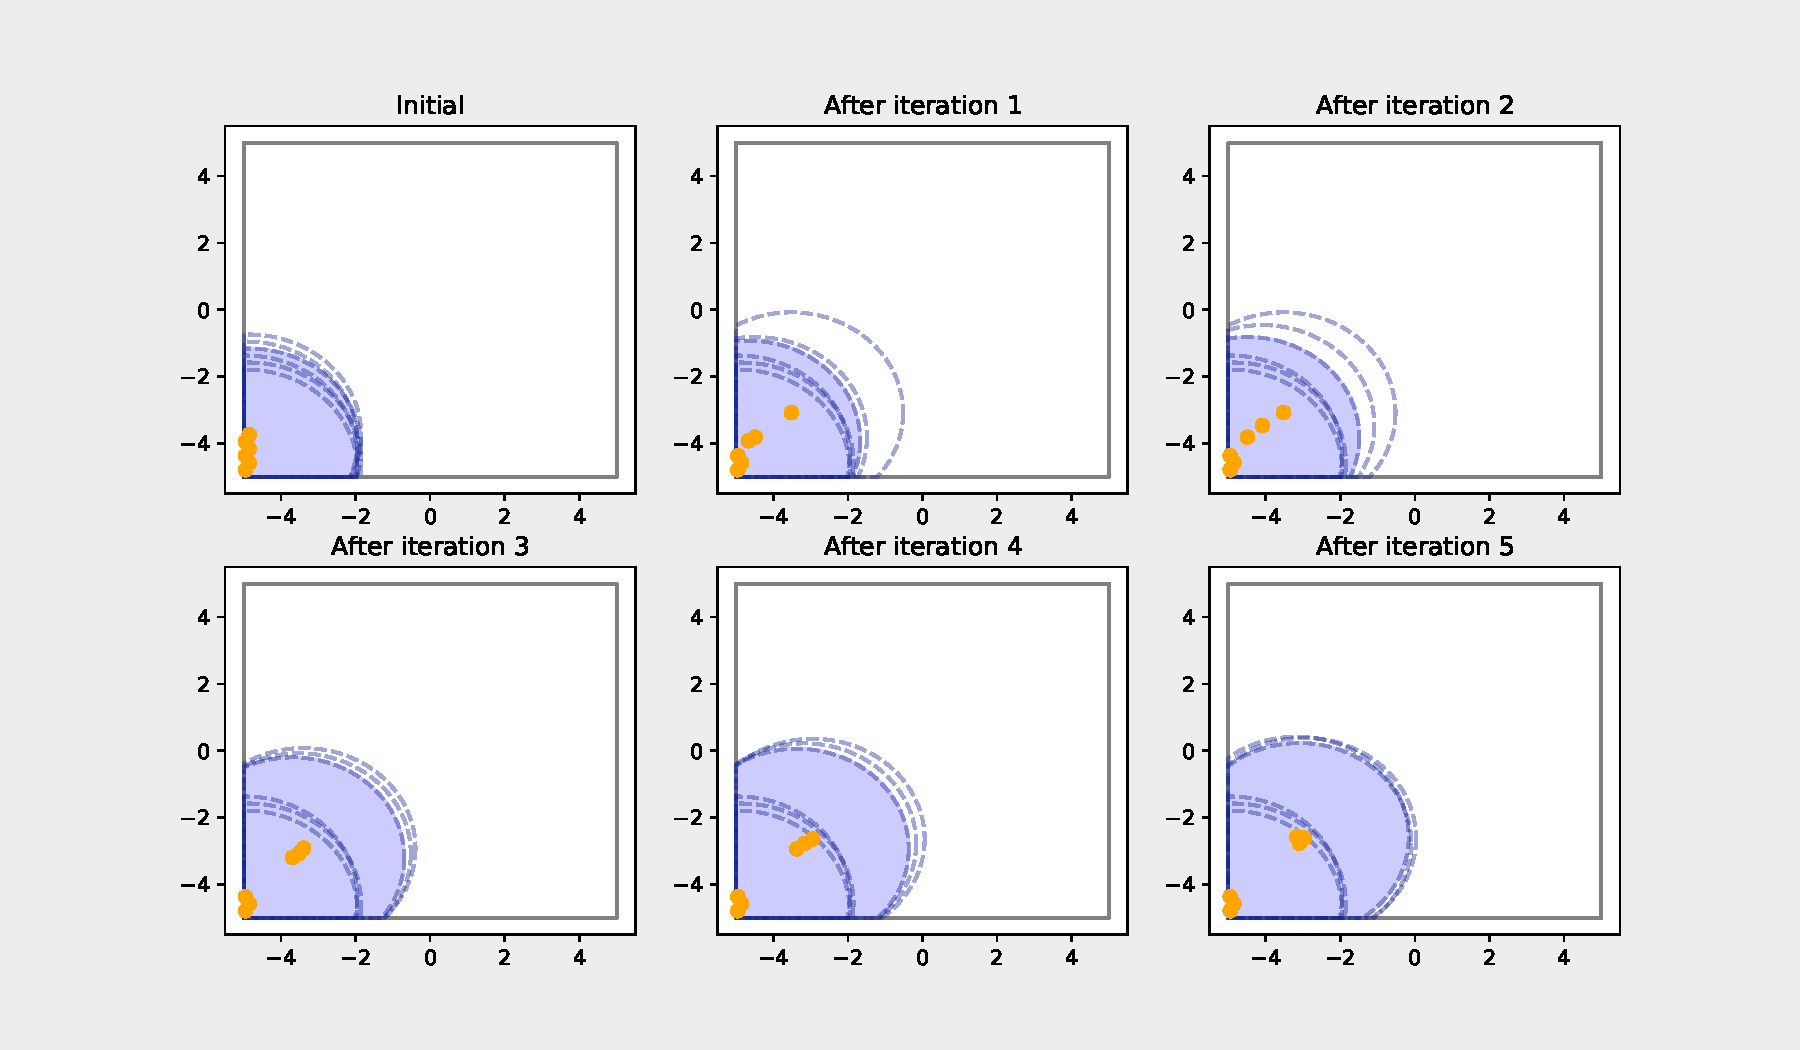
\includegraphics[width=\textwidth]{figs/bigworld_6_agnt_k_1_0_k_2_1_x_traj.pdf}
  \caption{Intermediate configurations for 6 agents in the Rectworld environment with $k_{1} = 0$ (no active dispersion).}
  \label{fig:bw_x_traj}
\end{figure}

Simulations performed in the Complexworld environment yet again show how active dispersion forces agents to explore the mission space. Without active dispersion Algorithm \ref{alg:alg1} converges quickly to a clearly sub-optimal
configuration as seen in \figref{fig:50_agnt_cw_k_1_0_k_2_1_distr}. Only a small portion of the swarm makes advancements into the mission space. Yet again this is caused by the majority of agents having a zero-gradient
local objective in every iteration of Algorithm \ref{alg:alg1} due to their visible sets being fully contained by those of at least three other agents. With active dispersion applied agents are explicitly encouraged to explore. Thus, as seen in \figref{fig:50_agnt_cw_k_1_1_k_2_1_distr}, agents disperse into the mission space and 
reach a far higher percentage of coverage than when no active dispersion is applied.

\subsection{Local convergence causing sub-optimal configurations}
For a swarm of 3 agents in the Rectworld environment, the final configurations obtained with 
and without active dispersion are shown in 
\Cref{fig:3_agnt_bw_k_1_1_k_2_1_distr} and \Cref{fig:3_agnt_bw_k_1_0_k_2_1_distr} respectively. The two configurations do not differ much, except that the configuration obtained when using active dispersion
is translated slightly to the north-east. As shown in \figref{fig:3_agnt_bw_k_1_0_s_traj} and \figref{fig:3_agnt_bw_k_1_1_s_traj} the agents make larger initial steps when active dispersion is applied. This
causes them to move further into the mission space. Thus less of their visual sets are clipped by the walls of the mission space, resulting in a larger percentage of covered area.

Both configurations obtained for 3 agents in the Rectworld environment exhibit the same problematic behavior. Moving the entire swarm in the north-east direction would yield a higher percentage of covered area,
but Algorithm \ref{alg:alg1} converges with the swarm placed so that the area covered by the three agents is clipped by the mission space walls. This is due to Algorithm \ref{alg:alg1} optimizing
the configuration of the swarm one agent at a time. In order to move the entire swarm to the north-east direction, all agents would have to move in the north-east direction, and they
would have to do so one at a time. In the configuration shown in \figref{fig:3_agnt_bw_k_1_0_k_2_1_distr} no single agent would increase their local objective by moving, although they would all benefit from each other moving.
Due to no single agent benefiting from moving, Algorithm \ref{alg:alg1} converges to a clearly sub-optimal configuration.

\figref{fig:6_agnt_bw_k_1_1_k_2_1_distr} shows the final configuration obtained for a swarm of 6 agents in the Rectworld environment using active dispersion. Again translating the
entire swarm north-east would give a higher percentage of coverage, but due to all agents being at local optima of their local objective functions, Algorithm \ref{alg:alg1} halts, and yields
a clearly sub-optimal configuration.